\documentclass[12pt, a4paper]{article}
 
% Russian-specific packages
%--------------------------------------
\usepackage[T2A]{fontenc}
\usepackage[utf8]{inputenc}
\usepackage[russian]{babel}
%--------------------------------------

% Extra packages
%--------------------------------------
\usepackage{diagbox}
\usepackage{pict2e}
\usepackage{keyval}
\usepackage{calc}
\usepackage{fp}
\usepackage{xcolor}
\usepackage{mathtools}
\usepackage{mathcmd}
\usepackage{cmap}
\usepackage{graphicx}
\usepackage{diffcoeff}
\graphicspath{{./images/}{./progs/pdf/}}
\usepackage[width=170mm, top=25mm, bottom=25mm]{geometry}
\everymath{\displaystyle}
%--------------------------------------

\begin{document}
	\begin{titlepage}
	\begin{center}
		\Huge
		\textbf{Практикум на ЭВМ}
		\vspace{0.5cm}
		
		\Large
		Аппроксимация задачи с помощью метода конечных элементов
		\vspace{1.5cm}
		
		\LARGE
		\textbf{Прокашев Максим Павлович}
		
		\vspace{0.5cm}
		\textbf{411 группа}
		
		\vspace{0.5cm}
		\today
		
		\vfill
		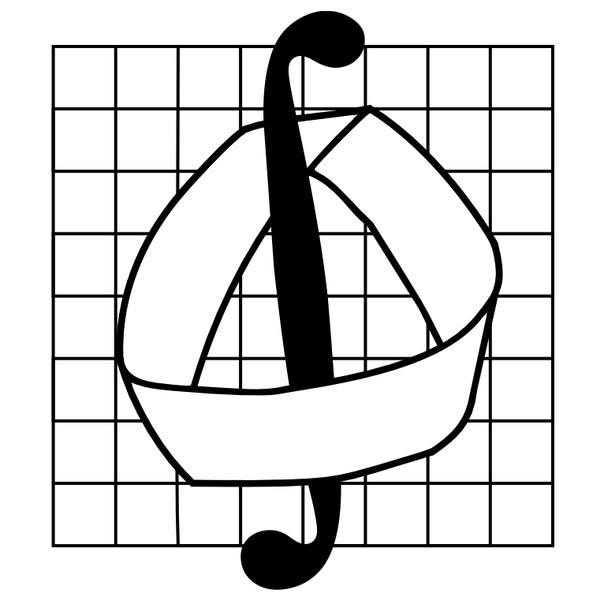
\includegraphics[width=6cm]{math_logo}
		\vspace{0.5cm}
		
		\Large
		2021
	\end{center}
\end{titlepage}
	
	\section{Условие задачи}
	\vspace{0.5cm}
	Для краевой задачи в единичном квадрате $\Omega$: \\
	\begin{equation*}
		\begin{cases}
			-\Delta u = f \\
			u|_{\delta \Omega} = 0
   		\end{cases}
 	\end{equation*} \\
 	построить проекционную схему при помощи неконформного метода конечных элементов и решить
 	полученную систему ЛАУ при помощи попеременно-треугольного метода.
 	
 	\section{Решение}
	\vspace{0.5cm}
	Квадрат $\Omega = \big[ 0, 1 \big] \times \big[ 0, 1 \big]$ разобьем квадратной сеткой
	с шагом $h = \frac{1}{n}$ и количеством элементов $n^{2}$:\\
	\begin{equation*}
		\{x_{ij} = (ih, jh) \ | \ i, j = 0, 1, \ldots, n \}
	\end{equation*}
	\begin{figure}[h]
		\centering
		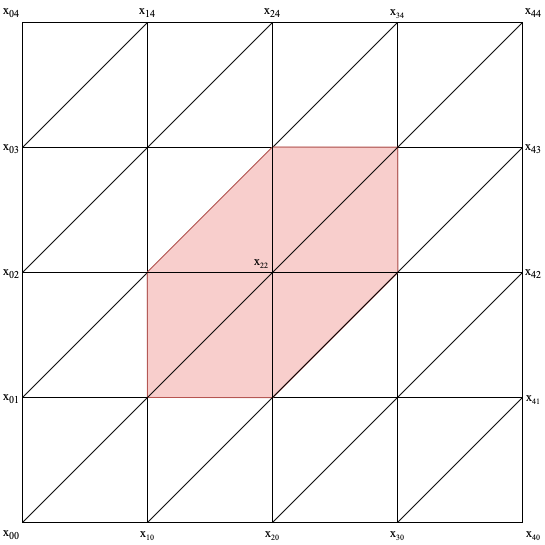
\includegraphics[width=9cm]{square_grid.png}
	\end{figure} \\
	Каждый элемент сетки разобьем диагональю из левого нижнего угла. 
	Таким образом получим триангуляцию единичного квадрата элементами
	$e_{i}, \ i = 1, \ldots, 2n^{2}$. \\
	Ищем решение $u(x,y)$ по методу Галеркина: 
	$u_{ij}(x) = \sum_{k,l=1}^{n-1} u_{kl} \phi_{kl} , \ u_{kl} = u(x_{kl})$ \\
	Интегральное тождество:
	$\int_{\Omega} \bigg( \diffp{u_{ij}}{x_{1}} \diffp{\phi_{ij}}{x_{1}} + \diffp{u_{ij}}{x_{2}} \diffp{\phi_{ij}}{x_{2}} \bigg) dx = \int_{\Omega} f \phi_{ij} dx$ \\\\\\
	Базисные функции: 
	$
	\phi_{kl}(x_{ij}) = 
		\begin{cases}
			1 \quad \text{если } x_{kl} = x_{ij} \\
			0 \quad \text{иначе}
		\end{cases}
	$ \\\\
	$\phi_{kl}$ --- непрерывны на $\Omega$, кусочно-линейные на треугольниках.
	Для любого внутреннего узла $x_{kl}$ базисная функция равна $0$ вне области шестиугольника,
	который образуют треугольники с вершиной в точке $x_{kl}$. 
	Пусть $\Omega_{kl}$ область шестиугольника в которой $\phi_{kl} \neq 0$. \\\\
	Посчитаем коэффициенты для разложения $u_{kl}$:
	\begin{itemize}
		\item Левая часть: 
		$a_{klmn} = \int_{\Omega} 
			\bigg( 
				\diffp{\phi_{kl}}{x_{1}} \diffp{\phi_{mn}}{x_{1}} + 
				\diffp{\phi_{kl}}{x_{2}} \diffp{\phi_{mn}}{x_{2}} 
			\bigg) dx_1 dx_2$
		\item Правая часть: $b_{kl} = \int_{\Omega} f \phi_{kl} dx_1 dx_2$
	\end{itemize}
	Для фиксированных $k, l$ левая часть не равна нулю только в $6$ случаях, 
	так как непустое пересечение с областью $\Omega_{kl}$ имеют только области:
	$\Omega_{k \pm 1, \ l}, \ \Omega_{k, \ l \pm 1}, \ \Omega_{k \pm 1, \ l \pm 1}$. \\
	Достаточно вычислить значение $\diffp{\phi_{kl}}{x_{1}}$ и $\diffp{\phi_{kl}}{x_{2}}$
	на $6$ треугольниках: \\\\
	\begin{equation*}
		\diffp{\phi_{kl}}{x_{1}} = 
			\begin{dcases}
				0            & \text{на } e_{1} \\
				-\frac{1}{h} & \text{на } e_{2} \\
				-\frac{1}{h} & \text{на } e_{3} \\
				0            & \text{на } e_{4} \\
				\frac{1}{h}  & \text{на } e_{5} \\
				\frac{1}{h}  & \text{на } e_{6}
			\end{dcases}
		\qquad \qquad \qquad
		\diffp{\phi_{kl}}{x_{1}} = 
			\begin{dcases}
				\frac{1}{h}  & \text{на } e_{1} \\
				\frac{1}{h}  & \text{на } e_{2} \\
				0            & \text{на } e_{4} \\
				-\frac{1}{h} & \text{на } e_{5} \\
				-\frac{1}{h} & \text{на } e_{6} \\
				0            & \text{на } e_{4}
			\end{dcases}
	\end{equation*} \\\\
	Тогда для фиксированных $k, l$:
	$
	\begin{cases}
		a_{k,l,k \pm 1,l \pm 1} = 0 \\
		a_{k,l,k \pm 1,l} = a_{k,l,k,l \pm 1} = -1 \\
		a_{k,l,k,l} = 4 \\
	\end{cases}
	$ \\\\\\
	Уравнение с номером $k, l$ имеет вид: \\
	\begin{equation*}
		\frac{4 u_{k,l} - u_{k-1,l} - u_{k,l-1} - u_{k+1,l} - u_{k,l+1}}{h^{2}} = 
			\frac{1}{h^{2}} \int_{\Omega_{kl}} f \phi_{kl} dx_1 dx_2
	\end{equation*} \\
	Аппроксимируем правую часть: 
	$
		\int_{\Omega_{kl}} f \phi_{kl} dx_1 dx_2 \approx
			f(x_{kl}) \int_{\Omega_{kl}} \phi_{kl} dx_1 dx_2 =
			f(x_{kl})h^{2} 
	$ \\\\
	Итоговое уравнение:
	\begin{equation*}
		\begin{dcases}
			\frac{4 u_{k,l} - u_{k-1,l} - u_{k,l-1} - u_{k+1,l} - u_{k,l+1}}{h^{2}} = f(x_{kl}) \\
			u_{0,l} = u_{n,l} = u_{l,0} = u_{l,n} = 0, \qquad l = 0, 1, \ldots, n
		\end{dcases}
	\end{equation*} \\\\\\
	Учитывая граничные условия, итоговая матрица размера $(n-1)^{2} \times (n-1)^{2}$ 
	имеет блочный вид и диагональную структуру: \\\\
	\begin{equation*}
	A =
		\begin{pmatrix}
			A_{1,1} & A_{1,2} & 0       & \cdots & 0           & 0           & 0           \\
			A_{2,1} & A_{2,2} & A_{2,3} & \cdots & 0           & 0           & 0           \\
			0       & A_{3,2} & A_{3,3} & \cdots & 0           & 0           & 0           \\
			\vdots  & \vdots  & \vdots  & \ddots & \vdots      & \vdots      & \vdots      \\
			0       & 0       &  0      & \cdots & A_{n-3,n-3} & A_{n-3,n-2} & 0           \\
			0       & 0       &  0      & \cdots & A_{n-2,n-3} & A_{n-2,n-2} & A_{n-2,n-1} \\
			0       & 0       &  0      & \cdots & 0           & A_{n-1,n-2} & A_{n-1,n-1}
		\end{pmatrix}
	\end{equation*} \\\\
	Матрицы $A_{ii}$ размера $(n-1) \times (n-1)$ имеют трехдиагональный вид: \\\\
	\begin{equation*}
	A_{ii} =
		\begin{pmatrix}
			4       & -1      & 0       & \cdots & 0      & 0      & 0      \\
			-1      & 4       & -1      & \cdots & 0      & 0      & 0      \\
			0       & -1      & 4       & \cdots & 0      & 0      & 0      \\
			\vdots  & \vdots  & \vdots  & \ddots & \vdots & \vdots & \vdots \\
			0       & 0       &  0      & \cdots & 4      & -1     & 0      \\
			0       & 0       &  0      & \cdots & -1     & 4      & -1     \\
			0       & 0       &  0      & \cdots & 0      & -1     & 4
		\end{pmatrix}
	\end{equation*} \\\\
	Матрицы $A_{ii \pm 1}$ размера $(n-1) \times (n-1)$ имеют диагональный вид: \\\\
	\begin{equation*}
	A_{ii \pm 1} =
		\begin{pmatrix}
			-1      & 0       & 0       & \cdots & 0      & 0      & 0      \\
			0       & -1      & 0       & \cdots & 0      & 0      & 0      \\
			0       & 0       & -1      & \cdots & 0      & 0      & 0      \\
			\vdots  & \vdots  & \vdots  & \ddots & \vdots & \vdots & \vdots \\
			0       & 0       &  0      & \cdots & -1     & 0      & 0      \\
			0       & 0       &  0      & \cdots & 0      & -1     & 0      \\
			0       & 0       &  0      & \cdots & 0      & 0      & -1
		\end{pmatrix}
	\end{equation*} \\\\\\\\\\\\

	\section{Результаты}
	\vspace{0.5cm}
	В качестве примера возьмем функцию: $f(x, y) = 2 \pi^{2} \sin(\pi x) \sin(\pi y)$. \\\\
	Аналитическое решение для этой задачи: $u(x, y) = \sin(\pi x) \sin(\pi y)$. \\\\
	Краевые условия выполнены: $u(0, y) = u(1, y) = u(x, 0) = u(x, 1) = 0$. \\\\
	Пусть $\widetilde{u}$ решение полученное методом конечных элементов, 
	а система ЛАУ решена при помощи попеременно-треугольного метода.
	Посмотрим на каком шаге при заданном $n$ достигается нужное значение квадратичной нормы. \\\\
	\begin{table}[h!]
	\renewcommand{\arraystretch}{1.3}
	\centering
 		\begin{tabular}{||c|| c c c c ||} 
 			\hline
 			\diagbox{\textbf{Норма}}{\textbf{n}} & \textbf{3} & \textbf{5} & \textbf{10} & \textbf{15} \\ 
 			\hline
 			\hline
 			\textbf{$\mathrm{e}{-4}$}  & 18  & 62  & 349  & 971  \\
 			\textbf{$\mathrm{e}{-5}$}  & 22  & 79  & 466  & 1339 \\
 			\textbf{$\mathrm{e}{-7}$}  & 30  & 112 & 699  & 2076 \\
 			\textbf{$\mathrm{e}{-10}$} & 43  & 163 & 1049 & 3180 \\
 			\textbf{$\mathrm{e}{-15}$} & 64  & 248 & 1633 & 5021 \\
 			\textbf{$\mathrm{e}{-20}$} & 85  & 333 & 2216 & 6862 \\
 			\textbf{$\mathrm{e}{-29}$} & 123 & 483 & ???? & ???? \\
 			\hline
 		\end{tabular}
	\end{table}
\end{document}